\documentclass[a4paper]{article}

%\usepackage{url}

%% Math
\usepackage{mathtools}
%% For Mengen like natural numbers
\usepackage{amsfonts}
%% Für spezielle Symbole
\usepackage{amssymb}

%% Images
\usepackage{import}
\usepackage{xifthen}
\usepackage{pdfpages}
%\usepackage{transparent}

%%% Command for simpler images
\newcommand{\incfig}[1]{%
    \def\svgwidth{\columnwidth}
    \import{./fig/}{#1.pdf_tex}
}

%% Links
\usepackage{hyperref}
\hypersetup{
    colorlinks=true,
    linkcolor=black,
    filecolor=magenta,
    urlcolor=cyan
}

%% Formatting
\usepackage{parskip}
\usepackage{pdflscape}

\title{Datenbanken \\ \large Bäckerei}
\author{Moritz Köhler und Niklas Reusch}

\begin{document}
\maketitle
\tableofcontents
\newpage

% Name der PDF Datei: Bäckereiprojekt_Köhler.pdf

% Arbeitszeiten
% 23.09 14:00-16:30
% 24.09 15:15-16:15
% 29.11 21:25-

\section{Anforderungsanalyse}

\begin{flushright}
Moritz Köhler \& Niklas Reusch
\end{flushright}

Um den Überblick über den Verkauf von zahlreichen Produkten einer Bäckerei-Kette zu behalten, müssen diese mit ihrem Produktname, dem zugehörigen Rezept, sowie dem Preis verwaltet werden. Hierbei soll ebenfalls hinterlegt werden, welche Produkte die verschiedenen Filialen der Bäckerei-Kette anbieten und welchen Zutatenbestand diese besitzen. Jede Filiale hat eine eigene Adresse und eine definierte Liste an Zulieferern, von welchen die Zutaten zu einem Festpreis in einer bestimmten Menge gekauft werden.  Da nicht immer in jeder Filiale alle Zutaten des Rezepts zur Produktherstellung vorhanden sind, wird ein Status hinterlegt (z.B. “herstellbar” oder “nicht herstellbar”). Außerdem können die Rezepte eines Produkts je nach Filiale unterschiedlich sein, weshalb es zu den Standard-Rezepten bestimmte Rezept-Varianten gibt. Für spezifischere Abweichungen des Standard-Rezepts soll für die Filialen das Hinzufügen eines Kommentars möglich sein. Zusätzlich hat jede Filiale eigene Mitarbeiter, welche mit ihrem Vornamen, Nachnamen, Adresse, Gehalt sowie dem Geburtsdatum verwaltet werden. Diese sind in bestimmte Schichten eingeteilt, welche zu einem bestimmten Datum und Uhrzeit starten und eine gewisse Dauer haben. Zusätzlich soll ein Überblick über die Verkaufszahlen gewährleistet sein. Hierzu wird eine Verkaufshistorie benötigt, welche zeigt, zu welchem Datum und Menge ein bestimmtes Produkt in einer Filiale verkauft wurde.

\begin{sloppypar}
Außerdem müssen verschiedene Benutzer verwaltet werden, welche unterschiedliche Informationen einsehen und verwalten. Zum einen gibt es die Mitarbeiter einer Filiale, welche ausschließlich Informationen zu den Produkten und Zutatenbeständen der jeweiligen Filiale einsehen und verwalten. Zum anderen gibt es den Filialleiter, welcher alle Informationen zur Filiale einsieht und verwaltet. Diese umfassen nicht nur Produktinformationen, sondern auch Informationen zu den Mitarbeitern, der Kauf- und Verkaufshistorie. Zu guter Letzt gibt es den Eigentümer der Bäckerei-Kette, welcher die Rolle des Administrators einnimmt. Dieser sieht alle Informationen über alle Filialen ein und verwaltet diese.
\end{sloppypar}

\section{ER-Modell}

\begin{flushright}
Niklas Reusch
\end{flushright}

% Wir müssen unsere Anforderungen für das ER Modell so erweitern, dass wir alle möglichen Beziehungen 
% Und wir brauchen ca. 10 Entitäten.

\pagebreak
\begin{landscape}
    %\begin{figure}[ht]
    %    \centering
    %    \def\svgwidth{\columnwidth}
    %    \import{./fig/}{ERM.pdf_tex}    % Text Scaling done within the .pdf_tex file
    %    \caption{ERM}
    %    \label{fig:ERM}
    %\end{figure}
    \begin{figure}[ht]
        \centering
        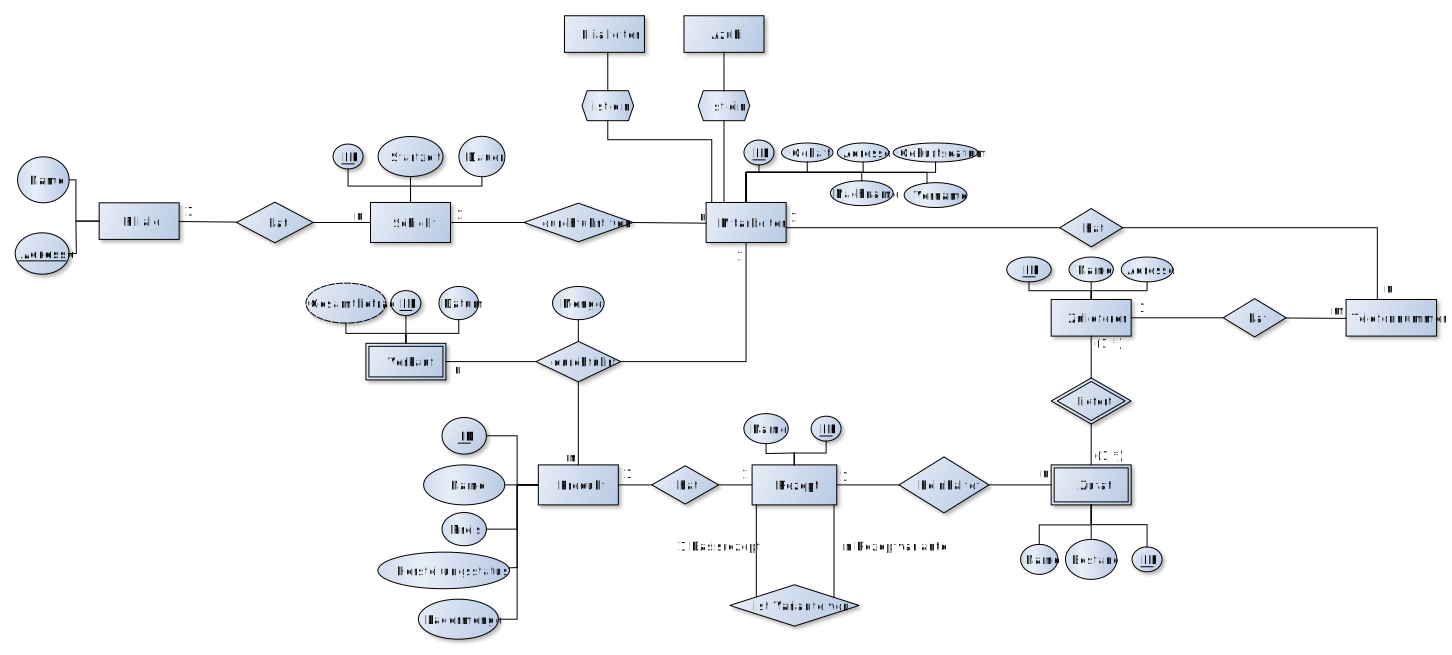
\includegraphics[width=2\textwidth]{./fig/ERM.png}
        \caption{ERM von Niklas Reusch}
        \label{fig:erm_from_niklas_reusch}
\end{figure}
\end{landscape}

\section{Relationale Modell}

\begin{flushright}
Moritz Köhler
\end{flushright}

% Für Normalisierung
% https://normalizer.db.in.tum.de/

\subsection{Entitäten}

Filiale: \{[\underline{FilialeID: integer}, Adresse: string, Name: string, LeiterID: MitarbeiterID]\}

Schicht: \{[\underline{SchichtID: integer}, Startzeit: datetime, Endzeit: datetime, FilialeID: integer]\}

Mitarbeiter: \{[\underline{MitarbeiterID: integer}, Gehalt: integer, Adresse: string, Geburtsdatum: datetime, Nachname: string, Vorname: string]\}

Azubi: \{[\underline{MitarbeiterID: integer}], Start: date, VerantwortlicherID: MitarbeiterID\}

MitarbeiterTelefonnummer: \{[\underline{Vorwahl: integer, Telefonnummer: integer}, MitarbeiterID: integer]\}

ZuliefererTelefonnummer: \{[\underline{Vorwahl: integer, Telefonnummer: integer}, ZuliefererID: integer]\}

Zulieferer: \{[\underline{ZuliefererID: integer}, Name: string, Adresse: string]\}

% Zutat ist eine Schwache Entität, kann aber von mehreren Zulieferern geliefert werden.
Zutat: \{[\underline{ZutatID: integer, ZuliefererID: integer}, Name: string, Bestand: integer, Einheit: string]\}

% Rekursiv
Rezept: \{[\underline{RezeptID: integer}, Name: string, Anleitung: text, Basis: RezeptID]\}

Produkt: \{[\underline{ProduktID: integer}, Name: string, Preis: integer, Status: integer, Lagerbestand: integer]\}

Verkauf: \{[\underline{VerkaufID: integer}, Datum: datetime, Gesamtbetrag: integer]\}

\subsection{Relationen}

durchgeführt-von: \{[\underline{SchichtID: integer, MitarbeiterID: integer}]\}

% beinhaltet: \{[\underline{RezeptID: integer, ZutatID: integer, ZuliefererID: integer}]\}
beinhaltet: \{[\underline{RezeptID: integer, ZutatID: integer}]\}

angeleitet: \{[\underline{ProduktID: integer, RezeptID: integer}]\}

verkauft: \{[\underline{ProduktID: integer, VerkaufID: integer}, Menge: integer, MitarbeiterID: integer]\}

\pagebreak
\subsection{Normalisierung bis 3NF}

%% Muss für die Aufgabe exemplarisch für ein nicht allzu einfaches dargestellt werden

Am Beispiel der Beziehung zwischen Mitarbeiter, Verkauf und Produkt. Siehe ERM Figure \ref{fig:erm_from_niklas_reusch}.

So gibt es diese große Relation (zur Übersicht habe ich die Typen weggelassen):

MVP: \{[MitarbeiterID, Gehalt, \dots, Nachname, ProduktID, Produktname, \dots, Lagerbestand, VerkaufID, Datum, Gesamtbetrag, Menge]\}

Mit den Folgenden Funktionalen Abhängigkeiten:

\begin{itemize}
    \item MitarbeiterID → Gehalt, \dots, Nachname
    \item ProduktID → Produktname, \dots, Lagerbestand
    \item VerkaufID → Datum, Gesamtbetrag
    \item VerkaufID, ProduktID → MitarbeiterID, Gehalt, \dots, Nachname, Produktname, \dots, Lagerbestand, Datum, Gesamtbetrag, Menge
\end{itemize}

Dies befindet sich in 1NF mit dem Kandidatenschlüssel (VerkaufID, ProduktID). Um diese in die 2NF zu überführen, wird die Kanonische Überdeckung genutzt.

\begin{enumerate}
    \item Linksreduktion
    \item Rechtsreduktion
    \item a → $\emptyset$
    \item FDs zusammenfassen
\end{enumerate}

Auf der Rechten Seite können nur die vierte Relation verkleinern:

\begin{itemize}
    \item VerkaufID, ProduktID → MitarbeiterID, Menge
\end{itemize}

Nun werde diese Funktionalen Abhängigkeiten in Relationen umgewandelt:

% Woher kommen die Kandidatenschlüssel?

\begin{enumerate}
    \item Mitarbeiter: \{[\underline{MitarbeiterID}, Gehalt, Adresse, Geburtsdatum, Nachname, Vorname]\}
    \item Produkt: \{[\underline{ProduktID}, Produktname, Preis, Status, Lagerbestand]\}
    \item Verkauf: \{[\underline{VerkaufID}, Datum, Gesamtbetrag]\}
    \item verkauft: \{[\underline{ProduktID, VerkaufID}, Menge, MitarbeiterID]\}
\end{enumerate}

Somit sind nun alle Nichtschlüsselattribute vollfunktional vom gesamten Schlüssel abhängig. Damit ist dies in 2NF.

Die Relationen die aus der Kanonischen Überdeckung entstehen sind die Grundlage für die Umwandlung in 3NF.

% TODO: Synthesealgorithmus muss ich nochmal besser aufschreiben.

\section{Datenschema in SQL}

\begin{flushright}
Niklas Reusch
\end{flushright}

\section{Entwurf}

\begin{flushright}
Moritz Köhler
\end{flushright}


\newpage
\section{Feedback}

\subsection{Feedback: ER-Modell}

\begin{flushright}
von Moritz Köhler für Niklas Reusch am 16.10.2025
\end{flushright}

Das ERM umfasst schon zum großteil die Anforderungen. Ergänzen kann man noch eine Spezifikation eines Mitarbeiter, den Filialleiter. Dieser leitet dann eine Filiale. Weitere Spezifikationen des Mitarbeiter können sein: Azubi, Besitzer.

Zum Azubi könnte man leicht eine Ternäre Beziehung hinzufügen, die auf der Spezialisierung aufbaut. Ein Mitarbeiter bringt einem Azubi ein Rezept bei.

Des weiteren lassen sich die Beziehungen Filiale führt einen Verkauf durch, Mitarbeiter führt einen Verkauf durch und Ein Verkauf enthält Produkte zu einer Ternäre Beziehung zusammenfassen. Die Attribute von der Entität Verkauf kannst du dann einfach an die Beziehung selbst schreiben.

Da Varianten eines Rezeptes selbst ein Rezept sind würde ich dort eine Rekursive Beziehung verwenden. Damit hätten wir dann auch eine Rekursive Beziehung in unserem ERM.

Ich bin mir bei der Rezept besteht aus Zutaten Beziehung etwas unsicher ob das tatsächlich eine "besteht aus" Beziehung ist.

Allgemein zum Format in yEd. Die Telefonnummer von Mitarbeiter und Zulieferer kann gerne mit nach oben, da diese unten mit den sehr Langen Verbindungen komisch aussieht. Es wäre auch schön, wenn die Abstände und Größen der Entitäten und Beziehungen gleich bleiben.

Bitte benutze für die Attribute auch das Attribut Feld unter dem Tab Entity Relationship statt dem Gelben aus Shapes. Für die Spezifikation kann man ein Sechseck aus BPMN benutzen und die Farben aus einer Entität kopieren. Dann sieht alles Einheitlich aus.

\subsection{Feedback: Relationale Modell}

\begin{flushright}
von Niklas Reusch für Moritz Köhler
\end{flushright}



\newpage
\subsection{Feedback: Datenschema}

\begin{flushright}
von Moritz Köhler für Niklas Reusch
\end{flushright}



\subsection{Feedback: Entwurf}

\begin{flushright}
von Niklas Reusch für Moritz Köhler
\end{flushright}



\end{document}